\documentclass[journal]{IEEEtran}
\usepackage[T1]{fontenc}
\usepackage[utf8]{inputenc}
\usepackage{amsmath,amssymb,bm}
\usepackage{booktabs}
\usepackage{graphicx}
\usepackage{multirow}
\usepackage{siunitx}
\usepackage{xcolor}
\usepackage{cite}
\usepackage[hidelinks]{hyperref}
\graphicspath{{figures/}}
\sisetup{detect-all,table-number-alignment=center}

\title{Missing EEG Channel Reconstruction Using Graph Signal Processing With Temporal Regularization}

\author{Carlos~Saldivia~Heinz%
\thanks{C. Saldivia Heinz is with the Department of Electronics, Universidad T\'ecnica Federico Santa Mar\'ia, Valpara\'iso, Chile.}}

\begin{document}
\maketitle

\begin{abstract}
Missing or corrupted electroencephalographic (EEG) channels can compromise spatial analyses and reduce usable recording time. Conventional spherical-spline interpolation uses sensor geometry but treats samples independently. This work formulates missing-channel recovery as reconstruction of a time-varying graph signal and combines a spatial graph-Laplacian prior with first-order temporal regularization. A fixed temporal-regularized Sobolev smoothing (TRSS) configuration was evaluated against the spherical-spline implementation in MNE-Python using exactly paired signals, masks, and random seeds. The frozen benchmark comprises 300 paired cases across two synthetic regimes, two PhysioNet EEG records, and the MNE Sample dataset, with random, neighboring, peripheral, and high-variance channel-removal patterns. Metrics were computed only on artificially hidden channels. Relative to spherical splines, TRSS achieved a 12.4\% median improvement in mean absolute error (95\% bootstrap interval: 7.8--17.4\%) and won 72.0\% of paired cases. Improvements were also observed for root-mean-square error, normalized RMSE, dynamic time warping, correlation, and $R^2$. However, spherical splines retained an advantage in log-spectral distance and were approximately 13.5 times faster at the median. Performance was heterogeneous: TRSS improved amplitude reconstruction in rough synthetic and real-data strata but underperformed on the smooth synthetic regime. These results support temporal graph regularization as a complementary reconstruction option rather than a universal replacement for spherical splines.
\end{abstract}

\begin{IEEEkeywords}
electroencephalography, missing channels, graph signal processing, temporal regularization, spherical splines, signal reconstruction.
\end{IEEEkeywords}

\section{Introduction}
\IEEEPARstart{E}{lectroencephalography} (EEG) records noninvasive electrical activity at multiple scalp locations. Its temporal resolution supports research and clinical workflows, yet the measurements remain vulnerable to electrode detachment, high impedance, motion, amplifier saturation, and localized artifacts. Removing an entire recording because a subset of channels is unusable wastes otherwise informative samples. Conversely, reconstructing a damaged channel without preserving spatial and temporal structure can distort downstream analyses.

The standard practical response is spatial interpolation. Spherical splines model scalp potentials as a smooth field over sensor locations \cite{perrin1989}, and their implementation in MNE-Python is widely available \cite{gramfort2013meg,gramfort2014mne}. This approach is computationally efficient and effective when the scalp field is sufficiently smooth. It does not, however, explicitly regularize temporal continuity while estimating each missing channel.

Graph signal processing (GSP) provides a natural representation in which electrodes are graph vertices, edge weights encode sensor proximity, and the voltage at each instant is a graph signal \cite{shuman2013,ortega2018}. Missing-channel interpolation can then be posed as graph-signal recovery \cite{narang2013}. For an EEG segment, the unknown is not a single graph signal but a matrix evolving over time. This motivates joint spatial and temporal regularization.

This paper evaluates temporal-regularized Sobolev smoothing (TRSS), a graph reconstruction model developed and audited in the accompanying thesis. The article is a new synthesis of the frozen thesis evidence; no additional reconstruction experiment is introduced. Its contributions are:
\begin{enumerate}
    \item a reproducible formulation that combines observed-channel fidelity, graph-Laplacian smoothness, and first-order temporal continuity;
    \item an exactly paired comparison against MNE spherical-spline interpolation over 300 cases and multiple missing-channel patterns;
    \item a multidomain assessment showing both the practical benefits and the failure modes of temporal graph regularization, including spectral-quality and runtime tradeoffs.
\end{enumerate}

The central claim is deliberately bounded. TRSS is not presented as a universal replacement for spherical splines, nor as clinically validated. The evidence supports it as a complementary method whose value depends on the signal regime, metric, and computational budget.
\section{Related Work}
\subsection{EEG Channel Interpolation}
Spherical splines remain a standard geometry-based approach for reconstructing scalp potentials \cite{perrin1989}. The method exploits the smoothness of the electrical field on a spherical head model and is available through established EEG software. Other spatial alternatives include radial basis functions \cite{jager2016rbf}. Such methods are attractive because they are interpretable, fast, and require no learned population model. Their main limitation for the present problem is that temporal dependence is not part of the reconstruction objective.

Data-driven EEG representations can exploit larger training collections, but they introduce model-training, distribution-shift, and data-governance considerations. The present work instead studies a deterministic, training-free regularizer. This distinction matters: the target is recovery of hidden channels in short multichannel segments, not generation of unconstrained EEG or replacement of artifact rejection.

\subsection{Graph-Based Reconstruction}
GSP generalizes classical signal concepts to irregular domains \cite{shuman2013,ortega2018}. Given a weighted graph, the combinatorial Laplacian quantifies variation across connected vertices. Low graph variation provides a prior for interpolation \cite{narang2013}. Graph construction is itself consequential; geometry-based graphs preserve an explicit, non-circular relationship to sensor layout, whereas data-derived graphs may encode statistical dependencies and can require separate training or leakage controls \cite{kalofolias_how_2016,shekkizhar2020}.

Time-varying graph-signal reconstruction extends this idea by coupling graph smoothness to evolution across samples. Sobolev-type formulations have been used for dynamic graph signals \cite{giraldo2022}. TRSS follows that general principle but uses a geometry-based EEG sensor graph and a simple first-difference temporal term, enabling direct comparison with a geometry-based spline baseline.
\section{Materials and Methods}
\subsection{Problem Formulation}
Let $\bm{X}\in\mathbb{R}^{N\times T}$ denote an EEG segment with $N$ channels and $T$ samples. The binary mask $\bm{M}\in\{0,1\}^{N\times T}$ is one for observed entries and zero for artificially hidden channels. Given the incomplete matrix $\bm{Y}=\bm{M}\odot\bm{X}$, the task is to estimate $\widehat{\bm{X}}$ while retaining observed values exactly.

Electrodes define the vertices of an undirected weighted graph $\mathcal{G}=(\mathcal{V},\mathcal{E},\bm{W})$. For sensor coordinates $\bm{r}_i$, each vertex is connected to its $k$ nearest neighbors, and geometry-derived weights decay with distance. With degree matrix $\bm{D}$, the combinatorial Laplacian is $\bm{L}=\bm{D}-\bm{W}$. This graph is fixed from sensor geometry and is not learned from hidden targets.

\subsection{Temporal-Regularized Sobolev Smoothing}
TRSS estimates the complete segment through
\begin{equation}
\begin{split}
\widehat{\bm{X}}=\arg\min_{\bm{Z}}\;&
\frac{1}{2}\lVert\bm{M}\odot(\bm{Z}-\bm{Y})\rVert_F^2 \\
&+\alpha\,\mathrm{tr}(\bm{Z}^{\mathsf T}\bm{L}\bm{Z})
+\beta\lVert\bm{Z}\bm{D}_t\rVert_F^2,
\end{split}
\label{eq:trss}
\end{equation}
where $\bm{D}_t$ is the first-order temporal difference operator. The first term enforces agreement with observed samples; the second penalizes graph variation; and the third discourages abrupt temporal changes. After optimization, observed entries are restored from $\bm{Y}$, making the observed-channel error identically zero by construction.

The confirmatory configuration was fixed at $k=4$, graph scale $\sigma=1.0$, $\alpha=0.8$, $\beta=0.15$, 120 iterations, and learning rate 0.05. These values were frozen before the final paired summary. Oracle-selected variants were analyzed in the thesis but are excluded from the principal claim because case-wise parameter selection is not a deployable comparator.

\subsection{Comparator}
The baseline was MNE-Python's EEG bad-channel interpolation with the spherical-spline option \cite{gramfort2013meg,gramfort2014mne}. This implementation reconstructs scalp potentials from sensor geometry following the spherical-spline principle \cite{perrin1989}. Both methods received the same signal, hidden-channel set, and sensor coordinates for each paired case.

\subsection{Evaluation Material and Missingness Design}
The frozen balanced benchmark contains five strata: a graph-smooth synthetic regime, a rougher synthetic regime, two records from the PhysioNet EEG Motor Movement/Imagery resource \cite{goldberger2000physiobank,schalk2004bci2000}, and the MNE Sample dataset. The synthetic strata provide controlled limiting cases; the real-data strata test transfer to recorded signals. This benchmark does not constitute clinical validation.

Four channel-removal patterns were applied: random channels, spatially neighboring channels, peripheral graph channels, and high-variance channels. Missingness levels comprised one channel, two channels, and 10\%, 30\%, or 40\% of available channels. Three random seeds were used. The Cartesian design produced 100 scenario clusters and 300 exactly paired cases. Scores were computed only on hidden channels.

\subsection{Outcome Measures and Uncertainty}
Amplitude fidelity was summarized with mean absolute error (MAE), root-mean-square error (RMSE), and normalized RMSE. Temporal shape was assessed with dynamic time warping (DTW) and mean correlation; explained variation with $R^2$; spectral behavior with signal-to-noise ratio (SNR), log-spectral distance (LSD), and mean coherence. Runtime per case represented computational cost.

For an error metric $e$ in which lower is better, relative improvement was $(e_{\mathrm{MNE}}-e_{\mathrm{TRSS}})/e_{\mathrm{MNE}}$; signs were reversed for higher-is-better metrics. We report paired win rates, median relative improvements, and cluster bootstrap 95\% intervals over the 100 scenario clusters. The interpretation emphasizes effect magnitude, heterogeneity, and practical tradeoffs rather than a binary significance decision.
\section{Results}
\subsection{Primary Paired Comparison}
Table~\ref{tab:primary} reports the fixed TRSS comparison against MNE spherical splines. Across 300 paired cases, TRSS reduced median MAE by 12.4\% (95\% bootstrap interval: 7.8--17.4\%) and won 72.0\% of cases (95\% interval: 63.7--79.3\%). Similar directional gains occurred for RMSE, NRMSE, DTW, correlation, and $R^2$.

\begin{table*}[t]
\caption{Fixed TRSS Versus MNE Spherical Splines in 300 Paired Cases}
\label{tab:primary}
\centering
\small
\begin{tabular}{@{}lrrrrrr@{}}
\toprule
Metric & MNE median & TRSS median & Median improvement & 95\% bootstrap interval & TRSS win rate & Win-rate interval \\
\midrule
MAE & $1.133\!\times\!10^{-5}$ & $8.462\!\times\!10^{-6}$ & 12.4\% & [7.8, 17.4]\% & 72.0\% & [63.7, 79.3]\% \\
RMSE & $1.474\!\times\!10^{-5}$ & $1.055\!\times\!10^{-5}$ & 13.9\% & [6.4, 19.3]\% & 70.3\% & [62.3, 78.0]\% \\
NRMSE & 0.725 & 0.634 & 13.9\% & [6.4, 19.3]\% & 70.3\% & [62.3, 78.0]\% \\
DTW & $6.732\!\times\!10^{-4}$ & $5.599\!\times\!10^{-4}$ & 9.8\% & [5.5, 12.7]\% & 71.0\% & [63.3, 78.7]\% \\
SNR & 9.466 & 10.029 & 3.7\% & [0.9, 9.6]\% & 61.0\% & [53.3, 68.3]\% \\
LSD & 0.751 & 0.767 & $-2.3$\% & [$-4.0$, $-0.2$]\% & 40.7\% & [32.3, 49.0]\% \\
Coherence & 0.887 & 0.888 & 0.2\% & [0.0, 0.5]\% & 58.3\% & [50.3, 66.0]\% \\
Correlation & 0.927 & 0.942 & 0.8\% & [0.3, 2.0]\% & 68.7\% & [60.7, 76.0]\% \\
$R^2$ & 0.475 & 0.598 & 16.9\% & [3.4, 52.8]\% & 70.3\% & [62.7, 78.3]\% \\
\bottomrule
\end{tabular}
\end{table*}

Fig.~\ref{fig:portfolio} makes the metric dependence explicit. The largest median relative gains occurred in $R^2$, RMSE/NRMSE, and MAE. In contrast, LSD favored spherical splines. Coherence improved only slightly, and its interval approached zero. Therefore, amplitude and temporal-shape improvement should not be interpreted as uniform spectral superiority.

\begin{figure*}[t]
\centering
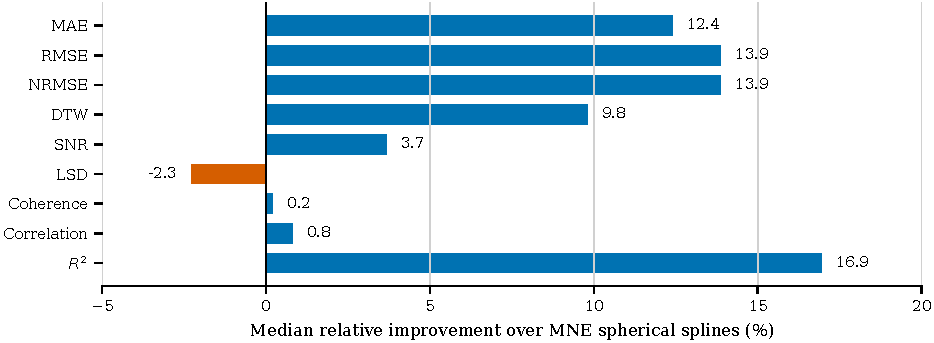
\includegraphics[width=0.94\textwidth]{metric_portfolio.pdf}
\caption{Metric portfolio for fixed TRSS relative to MNE spherical splines. Positive values favor TRSS; negative values favor MNE. Values are median paired relative improvements from the frozen thesis benchmark.}
\label{fig:portfolio}
\end{figure*}

\subsection{Heterogeneity Across Data Strata}
The aggregate result concealed a meaningful regime dependence (Fig.~\ref{fig:datasets}). TRSS won all rough-synthetic cases and achieved a 21.5\% median MAE improvement. It also improved median MAE for both PhysioNet records and the MNE Sample segment, with win rates from 73.3\% to 85.0\%. In the smooth synthetic regime, however, TRSS had a $-12.7$\% median MAE improvement and won only 20.0\% of cases. Spherical splines are well matched to that deliberately smooth spatial field, whereas the extra temporal prior can overconstrain the solution.

\begin{figure*}[t]
\centering
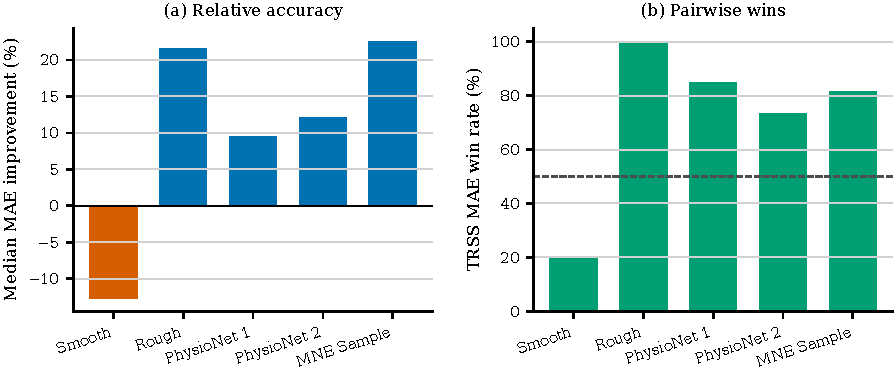
\includegraphics[width=0.94\textwidth]{dataset_summary.pdf}
\caption{Heterogeneity of fixed-TRSS MAE performance across benchmark strata. (a) Median paired MAE improvement relative to MNE; positive values favor TRSS. (b) Fraction of paired cases won by TRSS; the dashed line denotes 50\%. Each stratum contains 60 cases.}
\label{fig:datasets}
\end{figure*}

\begin{table}[t]
\caption{MAE Results by Benchmark Stratum}
\label{tab:dataset}
\centering
\small
\begin{tabular}{@{}lrrr@{}}
\toprule
Stratum & $n$ & Median improvement & Win rate \\
\midrule
Smooth synthetic & 60 & $-12.7$\% & 20.0\% \\
Rough synthetic & 60 & 21.5\% & 100.0\% \\
PhysioNet S1 & 60 & 9.5\% & 85.0\% \\
PhysioNet S2 & 60 & 12.2\% & 73.3\% \\
MNE Sample & 60 & 22.6\% & 81.7\% \\
\bottomrule
\end{tabular}
\end{table}

\subsection{Computational Tradeoff}
Median runtime was 0.121~s per case for fixed TRSS and 0.009~s for MNE, corresponding to an approximately 13.5-fold ratio. Fig.~\ref{fig:runtime} summarizes the accuracy--cost tradeoff. TRSS occupies the lower-error but higher-cost region. The absolute time remained below one second in this offline benchmark, but the difference is relevant for long recordings, repeated parameter search, and real-time systems.

\begin{figure}[t]
\centering
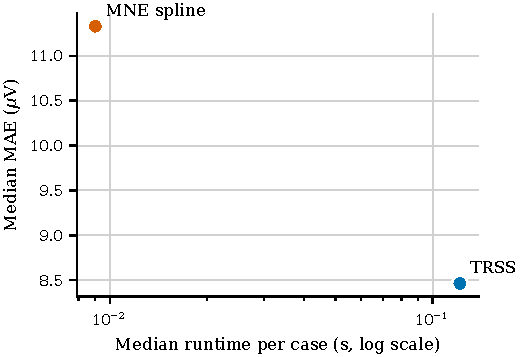
\includegraphics[width=\columnwidth]{runtime_tradeoff.pdf}
\caption{Median MAE--runtime tradeoff. Runtime is shown on a logarithmic scale. TRSS reduced median MAE at substantially greater computational cost.}
\label{fig:runtime}
\end{figure}
\section{Discussion}
The paired benchmark supports three main observations. First, a geometry-based graph model with explicit temporal regularization can improve recovery of hidden EEG channels on several amplitude and shape measures. Fixed TRSS improved median MAE, RMSE, NRMSE, DTW, correlation, and $R^2$, and its MAE advantage appeared in each evaluated real-data stratum. Because signals, masks, and seeds were shared between methods, these differences are not attributable to unequal missingness draws.

Second, the benefit is conditional. The smooth synthetic regime strongly favored spherical splines, and LSD favored MNE in the pooled comparison. These findings are coherent with the model assumptions. Spherical splines impose a spatially smooth scalp field and are difficult to improve upon when that assumption closely matches the generating process. TRSS trades additional temporal consistency against potential oversmoothing or spectral attenuation. Accordingly, method choice should depend on the intended downstream feature: lower pointwise error does not guarantee better preservation of every spectral property.

Third, robustness carries a computational cost. The fixed iterative solver was approximately 13.5 times slower at the median than the optimized MNE routine. The absolute runtime may be acceptable for offline repair of short segments, but MNE remains advantageous when latency, throughput, or simplicity dominates. Closed-form solvers, sparse factorization reuse, adaptive stopping, and warm starts are plausible engineering improvements, but they were not evaluated here.

\subsection{Practical Interpretation}
The results suggest a conservative decision rule. Spherical splines remain a strong default for smooth fields and time-critical processing. TRSS is most defensible when missingness is difficult, amplitude/shape fidelity is central, and a short segment provides sufficient temporal context. Reporting should include both an amplitude-domain measure and a spectral measure, since either alone can hide a relevant failure mode.

The method reconstructs channels; it does not identify whether a channel is bad. A separate quality-control procedure must define the channels to hide. Moreover, reconstruction should be logged and retained as a preprocessing transformation. It must not be represented as measured data, particularly in clinical or regulatory settings.

\subsection{Limitations}
The real-data component is limited to two PhysioNet records and one MNE Sample segment. Although the design spans 300 paired masks and several missingness modes, masks are not independent participants; uncertainty was therefore clustered by scenario rather than interpreted as population-level clinical uncertainty. The evaluation does not establish generalization across laboratories, montages, pathologies, amplifiers, or recording durations.

The sensor graph was derived from geometry and used fixed hyperparameters. This improves auditability but may be suboptimal for individual recordings. Conversely, per-case oracle selection would overstate deployable performance and was not used for the main result. The benchmark also compared against one established spline implementation rather than every interpolation or learning-based alternative.

Finally, artificial channel hiding provides known ground truth but is not identical to naturally corrupted electrodes. Natural failures can co-occur with bridging, reference changes, saturation, or spatially diffuse artifacts. Prospective evaluation on independently adjudicated failures and assessment of downstream biomarkers or classifiers are needed before clinical claims can be made.
\section{Conclusion}
Temporal-regularized graph reconstruction improved missing-channel EEG recovery over MNE spherical splines on several amplitude and temporal-shape measures in a 300-case paired benchmark. The fixed TRSS method achieved a 12.4\% median MAE improvement and a 72.0\% pairwise win rate, with favorable results in the evaluated real-data strata. The advantage was not universal: spherical splines performed better on a smooth synthetic regime, preserved log-spectral distance more consistently, and ran substantially faster. TRSS should therefore be viewed as a complementary, auditable reconstruction option whose use depends on the signal regime, target metric, and computational budget. Broader participant-level and naturally corrupted-channel validation remains necessary.

\IEEEtriggeratref{6}
\bibliographystyle{IEEEtran}
\bibliography{bibliography/references}
\end{document}
